\chapter{\sffamily Multi-stage pipelines}

{\bfseries\sffamily Concept.} To define and develop an archetype simulation environment for multi-stage pipelines. In our classification scheme, this archetype is defined by an arbitrary, directional state partition graph topology and would make sense for simulations of logistics problems or data processing pipelines. We will also discuss the typical ways in which the stages within the pipeline may only partially be observed in realistic examples, and analyse how best to deal with each situation. For the mathematically-inclined, this chapter will define the mapping of our formalism to multi-stage pipelines. For the programmers, the software which is designed and described in this chapter can be found in the public Git respository here: \href{https://github.com/worldsoop/worldsoop}{https://github.com/worldsoop/worldsoop}.


\section{\sffamily Defining the archetype}

The multi-stage pipeline archetype refers to simulation environments with a directional state partition graph with arbitrary connection topology. In this case, each state partition corresponds to a separate stage in some pipeline model of the real-world phenomenon. Directionality in the connection structure is the key distinction between this archetype and the others in our classification scheme. We've provided one illustrated example of a multi-stage pipeline state partition graph in Fig.~\ref{fig:state-partition-graph-multi-stage-pipelines}.

\begin{figure}[h]
\centering
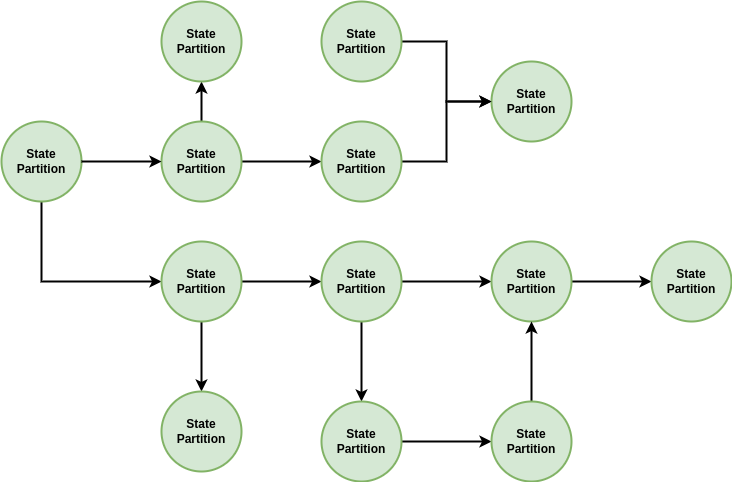
\includegraphics[width=12cm]{images/chapter-9-state-partition-graph.drawio.png}
\caption{State partition graph topology for multi-stage pipeline archetypes.}
\label{fig:state-partition-graph-multi-stage-pipelines}
\end{figure}

We're now ready to discuss how multi-stage pipelines are typically observed with data from realistic scenarios. To do this, it will help to first consider which real-world problem domains are best-suited to this archetype structure. From the literature, we can identify these as:
%%
\begin{itemize}
\item{Simulations of human logistics pipelines, e.g., organised supply chains~\cite{yan2022reinforcement}, humanitarian aid distribution pipelines~\cite{yu2021reinforcement}, hospital capacity planning~\cite{shuvo2021deep}, etc. }
\item{Environments which emulate data pipeline optimisation problems~\cite{nagrecha2023intune}.}
\end{itemize}
%%

\textcolor{red}{Within this topological archetype there will also be other categories to think are applicable:
\begin{itemize}
\item{Types of observation that can be made about the state.}
\item{Types of action that can be taken by an agent.}
\item{Types of agent? How frequently do these actions get taken? On what part of the state?}
\end{itemize}
}


\textcolor{red}{Types of actor:
\begin{itemize}
\item{sports team manager and other game player 1. substitute players 2. changes to tactics}
\item{public health authority and wildlife/national park control authority and livestock/crop farmer 1. spatially detect disease or damage 2. change state of a subset of the population}
\item{brain doctor and traffic light controller and city infrastructure maintainer 1. change the state of a subset of nodes in the network}
\item{supply/relief chain controller and hospital logistics manager and data pipeline controller 1. modify the relative flows between different pipeline stages}
\item{financial/betting/other market trader and market exchange mediator 1. interact with the market using an agent or collection of agents}
\end{itemize}}

\section{\sffamily Writing the code}